\documentclass[output=paper]{langsci/langscibook} 
\ChapterDOI{10.5281/zenodo.5675857}

\author{Anna Kurek-Przybilski\affiliation{Adam Mickiewicz University Poznań}}
\title{Generics as a paradigm: A corpus-based study of Norwegian}
\abstract{This paper examines generics as a part of human cognition, rooted in speakers' language knowledge in form of a grammatical paradigm. The paradigm proposed in this paper is based on a broader understanding of the notion, as presented in \citet{Diewald2009} and \citet{DiewaldSmirnova2010} among others. The matrix of the noun forms used in Norwegian in generic contexts is based on the models proposed by \citet{Radden2007,Radden2009} and \citet{Pettersson1976}. The models of generics were adjusted to the data from the Norwegian language, collected in this corpus-based study.}

\begin{document}
\maketitle
\section{Introduction}
For many years, a \textit{paradigm} was only associated with inflectional paradigms and morphology. However, a discussion on the matter in recent years has resulted in a new view on paradigms, a view that allows for a much broader understanding of the notion and the one that exceeds the branch of morphology.

The core of this paper is based on this new approach to grammatical paradigms which can be applied in examining different language phenomena. In this introductory section, the following questions will be addressed:

\begin{enumerate}[noitemsep]
    \item What is a paradigm in a broader sense?
    \item How will the paradigms proposed by \citet{Radden2007,Radden2009} and \citet{Pettersson1976} be modified when it comes to Norwegian?
    \item How can a paradigm be used with generics?
\end{enumerate}

%%% the text below was revised %%%
In scholarly literature, one finds numerous mentions of paradigms, most of them understood as morphological systems. An example of that can be found for instance in \citet[55]{AckermanBlevinsMalouf2009}, where paradigms are presented in a classic understanding of the term, namely as inflectional paradigms.

However, in this paper a different approach will be taken into account. \citet{Diewald2009} and \citet{Nørgård-Sørensen2011} present a new view on paradigms, which will be discussed and utilised in this study.

In her discussion, \citet[445]{Diewald2009} interprets paradigms as a representation of particular construction types. She points out that certain paradigms are obligatory, such as inflectional paradigms, whereas others are not. Genericity falls certainly in the second category -- it can be expressed in many different ways and even though certain NP types occur in certain generic contexts, they are not limited to only such contexts.

Such an understanding of the notion allows for a claim that certain language phenomena, such as genericity, can in fact be rooted in speakers' language knowledge and consist of a well-organised system of available forms. One can therefore differentiate between the different forms and the interpretations they imply. Nevertheless, the obligatoriness of such a paradigm remains questionable.

Paradigms understood in a broader sense were also discussed by \citet{Nørgård-Sørensen2011}. An example of Danish verbs that can be construed in different ways was provided by \citet[72--73]{Nørgård-Sørensen2011}. For instance, the verb \textit{skyde} `to shoot' can occur with a direct object or with a preposition \textit{på} `at'. The same mechanism can be observed in the case of generics, especially when it comes to bare nouns (BNs) occurring in generic contexts. In Norwegian (and Swedish, which will be discussed later), where BNs are common, certain verbs can require BNs:

\ea
\label{ex:norwegian-gen1}
	\gll Hun er lærer. \\
		 she is teacher-∅ \\
	\glt `She is a teacher.'
\ex \label{ex:norwegian-gen2} 
	\gll Det er sunt å ha hund. \\
		 it is healthy to have dog \\
	\glt `It is healthy to have a dog.'
\z

The verb `to be' in \REF{ex:norwegian-gen1} requires a BN because professions, nationalities and religious beliefs are expressed without any article in Norwegian (cf. Swedish as discussed by \citealp{Pettersson1976}). This can be considered an obligatory paradigm that follows certain grammar rules. In contrast to this, example \REF{ex:norwegian-gen2} shows a paradigmatic use of a BN with the verb `to have'. Here the BN functions as a concept of a dog, not a certain dog or a dog as the whole species. However, it is possible to say \textit{å ha en hund} `to have a dog', which does not change the meaning of the phrase. The examples illustrates therefore that certain paradigms, including the paradigm of genericity, are optional but nevertheless they structure the language.

\begin{sloppypar}
Another notion connected to paradigms understood in a broader sense is paradigmaticity. According to \citet[447]{Diewald2009}, paradigmaticity is an essential property that distinguishes grammatical items from lexical ones. This view can also be found in \citet{DiewaldSmirnova2010}, where paradigmaticity and obligatoriness are perceived as vital elements of the grammaticalisation process, based on the model of Lehmann.
\end{sloppypar}

In his seminal work on grammaticalisation, Lehmann presents parameters of grammaticalisation. One of those parameters is paradigmaticity.

\begin{quote}
    What is meant here by paradigmatic cohesion or paradigmaticity is the formal and semantic integration both of a paradigm as a whole and of a single subcategory into the paradigm of its generic category. This requires that the members of the paradigm be linked to each other by clear-cut paradigmatic relations, especially opposition and complementarity. \citep[141]{Lehmann2015}
\end{quote}

The main requirement when it comes to Lehmann's model is the clear-cut relation between the elements of a paradigm. Complementarity or opposition might not seem as clear-cut in case of generics and different noun forms used with generic NPs. However, analysing generics in texts where a broader context was provided, proved that certain noun forms complement each other in some contexts or exclude each other in other contexts.

The theoretical framework used in this paper is based on \citet{Diewald2009,DiewaldSmirnova2010} and \citet{Lehmann2015}. The approaches to grammatical paradigms presented in those studies will be combined with empirical data of Norwegian in order to evaluate the existing paradigms of generics proposed by \citet{Radden2007,Radden2009} and \citet{Pettersson1976}. The models will be discussed in greater detail in the following section. 

Genericity is a language phenomenon that is present in every language studied to date \citet{Behrens2000,Behrens2005}. However, there are no language devices used to express that phenomenon, despite the numerous theories on the matter \citep{Liebesman2011,Collins2018}. Certain researchers claim that a silent \textsc{gen}-operator exists (\citealp{Carlson1977,Carlson1982} and \citealp{Chierchia1998} among others), whereas others opt for the so-called ``simple view'' on generics \citep{Liebesman2011} that does not take into account any operators and treats generics in the same way as quantified statements. Nevertheless, no empirical studies have shown the presence of a device that would be used solely to express genericity, even though numerous studies on the matter show that the phenomenon may be one of the language universals, present already in children's speech (\citealp{Gelman-Tardif1998, LeslieGelman2012} among others).

In different studies concerning generics, the following claims on the paradigmatic nature of the phenomenon are made:

\begin{enumerate}
    \item Genericity depends on one's cognitive competences \citep[35]{Collins2018}.
    \item Genericity is a linguistic universal \citep[381]{Leslie2007}.
    \item Genericity is an internal paradigm, rooted in speakers' knowledge about the world \citep{Gelman-Tardif1998,Leslie-etal2011}.
\end{enumerate}

When it comes to the first claim, the fact that generics depend on one's cognition is closely connected to the paradigmatic view on the matter. Being able to interpret and produce generic NPs, sentences and texts means that certain aspects of the phenomenon are automatised -- be it on the cognitive level or on the grammatical level.

Another claim is that genericity is a linguistic universal, as is proposed by \citet{Leslie2007}. Indeed, numerous studies confirm that children at a very early age are able to correctly interpret and produce generic statements \citep{Gelman-Tardif1998}. This can also imply that generic knowledge is deeply rooted in one's cognition in the form of a paradigm \citep{Leslie-etal2011}.

In the cognitive literature on the matter, one finds numerous studies with different models of genericity. For instance, \citet{Leslie-etal2011} present a model of generic predications and types of references that may be construed with them in English. The model is based on the truth-value of the predications and can be applied when analysing generic sentences.

As has been mentioned, the models of generics that will be utilised in this study and modified according to the data, are those proposed by \citet{Radden2007,Radden2009} and \citet{Pettersson1976}. The first two models are based on English where four noun forms can be used to express genericity, namely indefinite singular, indefinite plural, definite singular and definite plural. The noun forms and their generic meanings according to Radden's model are depicted in \tabref{tab:Radden2009}.

\begin{table}
\footnotesize
\caption{Types of generic reference (Table 2 in \citealt[224]{Radden2009}.)\label{tab:Radden2009}}
\begin{tabularx}{\textwidth}{ lll >{\raggedright}p{\widthof{exclusive/}} Q }
\lsptoprule                                                               
    & generic type            & generic form        & ex-/inclu\-siveness    & generic meaning \\\midrule
(a) & representative generic  & indefinite singular & exclusive            & arbitrary instance  representing its type\\\tablevspace
(b) & proportional generic    & indefinite plural   & exclusive\slash inclusive  & salient proportion of the    type’s reference mass\\\tablevspace
(c) & kind generic            & definite singular   & inclusive            & prototypical subtype of  a well-established type\\\tablevspace
(d) & delimited generic       & definite plural     & inclusive            & delimited human set  within a domain\\
\lspbottomrule
\end{tabularx}
\end{table}

All types of genericity are illustrated by \citet[224]{Radden2009} as follows:

\begin{exe}
    \ex A lion has a bushy tail. \hfill{representative generic} \label{ex:lion1}
    \ex Hedgehogs are shy creatures. \hfill{proportional generic} \label{ex:hedgehog2}
    \ex The tiger hunts by night. \hfill{kind generic} \label{ex:tiger3}
    \ex The Italians love pasta. \hfill{delimited generic} \label{ex:italians4}
\end{exe}

\noindent In the example \REF{ex:lion1}, a member of the kind represents the whole species, indicating that having a bushy tail is a characteristic feature of most lions. Proportional generic is depicted with example \REF{ex:hedgehog2} and it concerns prototypical members of the kind. Namely, most hedgehogs are shy and therefore the feature can be connected to the whole kind. In example \REF{ex:tiger3} a reference to a kind is expressed with the use of indefinite singular NP. Kind-reference rarely allows for exceptions, therefore one may assume that a great majority of tigers hunts by night. The last category of generic expressions in English, namely delimited generic, is limited to human groups only, as can be seen in example \REF{ex:italians4}. The definite plural generic in English cannot be used with other nouns, whereas in Norwegian this NP type occurs in many more generic contexts as will be discussed later in this paper.

A graphic representation of English generics is presented in \figref{fig:types-radden2007}.

\begin{figure}
	\caption{Types of generic reference (Table 5.4 in \citealt[111]{Radden2007}).\label{fig:types-radden2007}}
	\includegraphics[width=.85\textwidth]{figures/Kurek-fig2mod.pdf}
\end{figure}

The generic noun forms, both definite and indefinite, singular and plural, have certain functions and interpretations assigned to them. For instance, indefinite singular is used when referring to a single member of a given group in order to state a generalisation about the whole species. A similar use is assigned to definite singular which is used mostly as a kind-reference. The two plural forms -- indefinite and definite -- also have their typical uses according to the proposed paradigm. Indefinite plurals are used when a certain proportion of members in a group (the majority) share a given feature, whereas the definite plural form is used only when talking about groups of people.

Both models proposed by \citet{Radden2007} and \citet{Radden2009} are constructed according to the restrictions mentioned by \citet{Lehmann2015}. Namely, the functions of generic forms are complementary and/or opposite to each other. This results also in relatively low interchangeability of the forms. For instance, delimited generics used solely when talking about people in English cannot be utilised as kind generic, and so on.

In both models, bare nouns are not taken into consideration as they are not very common in generic contexts in English. The only situation when BNs are used generically is with mass nouns. However, generic use of this noun type in Norwegian (and Swedish as will be presented) is a lot more frequent.

Let us now consider the paradigm of Swedish generics proposed by \citet{Pettersson1976} in \figref{fig:Pettersson_graph},\footnote{My translation into English. For the original graph in Swedish the reader is referred to the mentioned paper \citep[121]{Pettersson1976}.} where BNs occur as one of the available generic forms.


\begin{figure}
	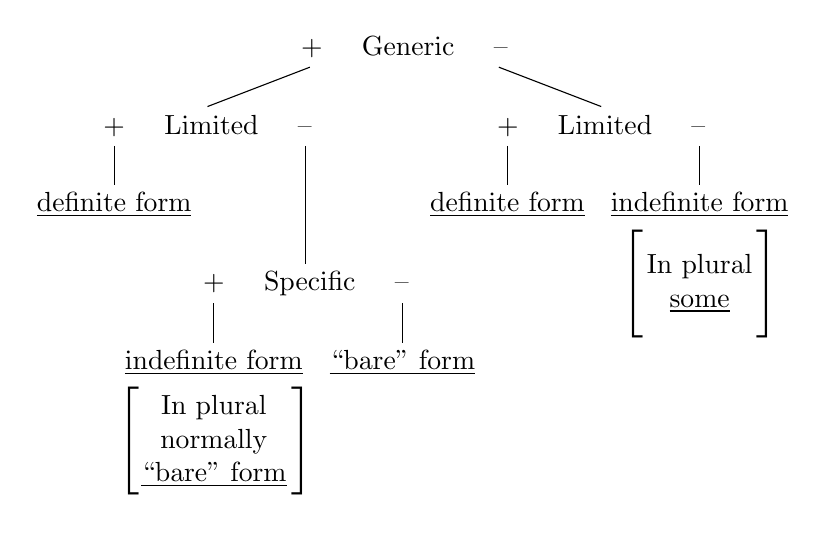
\begin{tikzpicture}
%	\draw[style=help lines] (0,0) grid (12,8);
	%Text coordinate
	\coordinate (generic) at (6,7) ;
	\coordinate (limited1) at (3.5,6) ;
	\coordinate (limited2) at (8.5,6) ;
	\coordinate (definite1) at (2.315,5) ;
	\coordinate (specific) at (4.75,4) ;		
	\coordinate (indefinite1) at (3.58,3) ;
	\coordinate (bare) at (5.975,3) ;		
	\coordinate (definite2) at (7.31,5) ;
	\coordinate (indefinite2) at (9.75,5) ;
	\coordinate (bracket1) at (3.58,2) ;
	\coordinate (bracket2) at (9.75,4) ;
		
	%Text
	\draw (generic) node{+\hspace{0.5cm}Generic\hspace{0.5cm}--};
	\draw (limited1) node{+\hspace{0.5cm}Limited\hspace{0.5cm}--};
	\draw (limited2) node{+\hspace{0.5cm}Limited\hspace{0.5cm}--};
	\draw (definite1) node{\underline{definite form}};
	\draw (specific) node{+\hspace{0.5cm}Specific\hspace{0.5cm}--};
	\draw (indefinite1) node{\underline{indefinite form}};
	\draw (bare) node{\underline{“bare” form}};
	\draw (definite2) node{\underline{definite form}};
	\draw (indefinite2) node{\underline{indefinite form}};
	
	%Lines
	\draw (4.8,6.75)--(3.5,6.25);%limited1
	\draw (7.2,6.75)--(8.5,6.25);%limited2
	\draw (2.315,5.75)--(2.315,5.25); %def1
	\draw (4.75,5.75)--(4.75,4.25);%specific
	\draw (3.58,3.75)--(3.58,3.25);%indefinite1	
	\draw (5.975,3.75)--(5.975,3.25);%bare
	\draw (7.31,5.75)--(7.31,5.25);%definite2
	\draw (9.75,5.75)--(9.75,5.25);%indefinite2
	
	\draw (bracket1) node[align=center]{In plural\\normally\\\underline{“bare” form}};
	\draw(2.5,2) node{\scalebox{1.3}{\Bigg[}};
	\draw(4.7,2) node{\scalebox{1.3}{\Bigg]}};
	
	\draw (bracket2) node[align=center]{In plural\\\underline{some}};
	\draw(8.9,4) node{\scalebox{1.3}{\Bigg[}};
	\draw(10.6,4) node{\scalebox{1.3}{\Bigg]}};
\end{tikzpicture}
\caption{Reference types in Swedish according to \citet[121]{Pettersson1976}\label{fig:Pettersson_graph}}
\end{figure}


The author proposes a number of possible readings of noun forms that can occur with generics. Such references are divided according to the features ``limited $+/-$'' and ``specific $+/-$'', according to which non-generic nouns are always specific \citep[121]{Pettersson1976}.

\citeauthor{Pettersson1976} provides also a number of examples that illustrate generics presented in his model:

\ea\label{ex:swedish1}
	\gll En hund jagar katter. \\
		 a dog chase cat.\textsc{pl} \\
	\glt `A dog chases cats.'
\ex\label{ex:swedish2}
	\gll En pojke gråter inte. \\
		 a boy cry not \\
	\glt `A boy doesn't cry.'
\ex\label{ex:swedish3}
	\gll Gärdsmygen är en flyttfågel.\\
		 wren.\textsc{def} is a migratory.bird \\
	\glt `The wren is a migratory bird.'
\ex\label{ex:swedish4}
	\gll Hunden skällar. \\
		 dog.\textsc{def} bark \\
	\glt `The dog barks.'
\ex\label{ex:swedish5}
	\gll Den svenske socialdemokraten lever och dör för sitt parti. \\
		 the swedish social.democrat live and die for his party \\
	\glt `The Swedish social democrat lives and dies for his party.'
\z
	
\noindent All of the sentences above are generic, even though they include two NP types~-- singular indefinite and singular definite. The examples in \REF{ex:swedish2} and \REF{ex:swedish4} illustrate representative generic, where a single instance represents the kind, namely `a dog' and `a boy' have some features that can be assigned to the whole group (most/all dogs chase cats and none/almost none boys cry).

\begin{sloppypar}
The examples \REF{ex:swedish3}, \REF{ex:swedish4} and \REF{ex:swedish5}, where definite singular NPs are used, can be seen as \textit{classic} kind references, where a prototypical instance represents the whole kind. One can assume that the prototypical wren shares a certain behaviour of all wrens, just as the prototypical dog does and the prototypical politician supporting the Social Democratic Party.
\end{sloppypar}

What is more, Pettersson's model allows for a bare form in non-specific contexts. Generic references are indeed considered non-specific, as they are generalisations, not references to particular instances of a given kind (cf. \citealp{Lyons1977}).

The examples of a non-specific use of bare nouns can be seen in the sentences below \citep[127]{Pettersson1976}:

\ea\label{ex:swedish6}
	\gll Han är lärare. \\
		 he is teacher \\
	\glt `He is a teacher.'
\ex\label{ex:swedish7}
	\gll Han är prest. \\
		 he is priest \\
	\glt `He is a priest.'
\z

\noindent Professions, nationalities and religious functions are used without articles in Swedish (as well as in Norwegian). The reason for this, as Pettersson explains, is that they describe general concepts. A similar statement can be said about bare generics in Norwegian, as in example \REF{ex:norwegian1}.

\ea\label{ex:norwegian1}
	\gll Ola vil kjøpe hus. \\
		 Ola will buy house \\
	\glt `Ola will buy a house.'
\z

\noindent The NP `house' is rather a concept than a particular house that Ola wants to purchase. The conceptual BNs in Norwegian are neither singular nor plural -- they are neutral when it comes to number, as well as definiteness (cf. \citealp{Halmoy2016}). They can also be used in generic contexts as will be shown later in the paper.

For the purpose of this study, all of the models presented above will be used to identify different types of generics in order to create a paradigm of the phenomenon in Norwegian. The following section focuses on the material used for the study, in Sections~\ref{sec:results} and~\ref{sec:discussion} the results of the analysis will be presented, whereas \sectref{sec:implications} concerns implications for further research in the field.

\section{Material}
\label{sec:material}
The study presented in this paper is based on a tailor-made corpus of generic texts. 170 texts (27 761 tokens in total) were retrieved from an online encyclopaedia \textit{Store norske leksikon}. The encyclopaedia contains texts written both in \textit{bokmål} and \textit{nynorsk}, the two written standards of Norwegian. In this study, only texts written in \textit{bokmål} are analysed.\footnote{The reason for such a choice is that the \textit{bokmål} language variant is used by the majority of the population (87.7\% according to a study published by \citealt{Riksmalsforbundet2017}).}

There were many reasons for the choice of encyclopaedic texts. First of all, generic NPs and sentences are not annotated in any of the available corpora of Norwegian so the phenomenon would have to be tagged manually anyway. Second of all, tagging genericity manually means that the texts chosen for the analysis must contain relatively many references of this sort in order for the material to be sufficient. This might not be the case should newspaper articles or literary texts be analysed, where the number of generic references is relatively low.

Finally, genericity is a context dependent phenomenon and it can occur both at the NP level, sentence level and text level \citep{Behrens2005}. Therefore, choosing the texts that are primarily generic makes the analysis possible, also when it comes to the available resources.

The texts chosen for the study are at least one paragraph long and contain at least one generic reference. The texts are divided into five thematic categories:

\begin{enumerate}
    \item people,
    \item animals,
    \item plants,
    \item tools,
    \item other.
\end{enumerate}

Below follow the example generic sentences from each of the categories:

\ea\label{ex:corpus1}
	\gll Vitnet skal som utgangspunkt gi forklaringen umiddelbart for den dømmende rett. \\
		 witness-\textsc{def} shall as rule give explanation-\textsc{def} immediately for the sentencing court \\
	\glt `A witness shall, as a rule, provide an explanation immediately to the sentencing court.'
\ex\label{ex:corpus2}
	\gll Måkene er hvite, grå og svarte. \\
		 seagull-\textsc{pl}.\textsc{def} are white gray and black \\
	\glt `Seagulls are while, gray and black.'
\ex\label{ex:corpus3}
	\gll Mammuttreet er en av de eldste levende organismer på Jorden. \\
		 giant.redwood-\textsc{def} is one of the oldest living organisms on Earth \\
	\glt `The giant redwood is one of the oldest living organisms on Earth.'
\ex\label{ex:corpus4}
	\gll Høvel er et verktøy til utjevning av treoverflater. \\
		 planer is a tool to even of wood.surface-\textsc{pl} \\
	\glt `A planer is a tool used to even wood surfaces.'
\ex\label{ex:corpus5}
	\gll En dal er en langstrakt fordypning i jordskorpen. \\
		 a valley is a enlongated deepening in earth.crust \\
	\glt `A valley is an elongated deepening in the Earth's crust.'
\z


The category `people' contains 20 texts, the categories `animals', `plants' and `tools' contain 25 texts each, whereas the category `other' consists of 75 texts. Differences in the number of texts in some of the categories is due to a few reasons. When it comes to the category `people', finding a description of an ethnic group, a nationality or an official function that is written in \textit{bokmål} and has the length of at least one paragraph, is a challenge. However, the difference of 5 texts in relation to the categories `animals', `plants' and `tools' is not significant in terms of the results.

The category `other' is the biggest of the whole corpus and it contains most diverse NP types. There are countable nouns and mass nouns, descriptions of objects, abstract notions, professions\footnote{Descriptions of professions are recognised as different from descriptions of groups of people. Professions are perceived more as concepts or a type of job, not people who perform a given task. Therefore the NPs of this sort are classified in the category `other' and not `people'. Official functions however, such as `king', `priest' etc. are classified in the category `people'.}, elements of the landscape and many others. Since the category contains so many different nouns that do not fit to any of the other categories, it also consists of many more texts. This way numerous generic contexts are taken into account without the need to divide the corpus into many separate subcategories.\largerpage

The choice of source texts for the analysis is subjective and its main purpose is to investigate the use of noun forms with different types of nouns -- animate, inanimate, countable and mass, as well as those recognised as well-established kinds (WEKs) and familiar nouns (c.f. \citealp{GenBook1995} and \citealp{Borthen2007} among others). 

The example sentences with each of those NP types can be found below (\REF{ex:animate}~-- animate, \REF{ex:inanimate_countable} -- inanimate and countable, \REF{ex:mass} -- mass noun and \REF{ex:WEK} -- WEK):

\ea\label{ex:animate}
	\gll Hunden var det første husdyret vårt. \\
		 dog.\textsc{def} was the first domestic.animal our \\
	\glt `The dog was our first domestic animal.'
\ex\label{ex:inanimate_countable}
	\gll Skruer har mange anvendelser og former. \\
		 screws have many uses and forms \\
	\glt `Screws have many uses and forms.'
\ex\label{ex:mass}
	\gll Blekk bestod opprinnelig av sot eller farger fra mineraler, planter og dyr. \\
		 ink consisted originally of soot or dyes from minerals, plants and animals \\
	\glt `Ink consisted originally of soot or dyes from minerals, plants and animals.'
\ex\label{ex:WEK}
	\gll Stavkirke er en høyt utviklet kirketype,. \\
		 stave.church-∅ is a highly developed church.type \\
	\glt `A stave church is a highly developed church type.'
\z


All texts in the corpus were tagged manually for genericity and noun forms of the NPs in question. The material was annotated and analysed with the use of R software (version 3.6.1). A random sample of annotated texts was proofread by a native speaker of Norwegian in order to eliminate potential mistakes or misinterpretations of generic references. However, due to the fact that all texts in the corpus are generic, annotating genericity was a fairly simple task and no mistakes were found in the randomly generated sample.

\section{General results}
\label{sec:results}
In the Norwegian nominal system, one finds five NP types, namely: BN (\textit{hund} `dog'), indefinite singular (\textit{en hund} `a dog') and plural (\textit{hunder} `dogs'), as well as definite singular (\textit{hunden} `the dog') and plural (\textit{hundene} `the dogs'). Among the five NP types, BNs seem to have the least stable status. In recent years, it has been discussed whether BNs are marked for number and definiteness. According to one view, they can be considered indefinite and singular \citep{Borthen2003}, whereas others claim that BNs are neutral in terms of definiteness and number (cf. \citealp{Halmoy2016}). As will be presented in this section, the second view seems to be more plausible. BNs are not considered singular or plural, neither are they considered (in)definite.


All nouns tagged as generic were counted and summed up in \tabref{tab:results}.

\begin{table}
\caption{Generic noun forms in the corpus -- general results\label{tab:results}}
\begin{tabular}{lrr} 
\lsptoprule  & $n$ & \%\\\midrule
    BN    &  345 & 39.66\\ 
    IndSg &   31 &  3.56\\
    DefSg &  185 & 21.26\\
    IndPl &  230 & 26.44\\
    DefPl &   79 &  9.08\\
\lspbottomrule
\end{tabular}
\end{table}
 
As can be seen, the three most frequently occurring noun forms include bare nouns, indefinite plural and definite singular. The two other forms, namely indefinite singular and definite plural, were used less frequently.
 
The main tendencies for the use of different noun forms already show that certain of them are used in many more contexts than other ones. For instance, BNs were used in numerous examples throughout all corpus texts, both as first mentions and as subsequent mentions. What is worth pointing out is that first mentions in many of the corpus texts were both encyclopaedic entries and subjects of the first sentences. This may be one of the reasons for such a frequent use of BNs. However, in many of the texts BNs appeared also as subsequent mentions, following often other noun forms used earlier in the text.

The second most often used noun form was indefinite plural, seen often as \textit{default} when it comes to expressing genericity in Germanic languages (cf. \citealp{Carlson1977,GenBook1995, Chierchia1998,Pettersson1976} among others). The collected data proves that this claim holds also for Norwegian (see \sectref{sub:indpl}).

Another aspect that was also observed in the corpus, was the position of generic NPs in the corpus texts. The results are shown in \tabref{tab:position}.
 
\begin{table}
\caption{Generic noun forms -- position in a sentence\label{tab:position}}
\begin{tabular}{lrr} 
\lsptoprule
                    & $n$    & \%  \\ 
   \midrule
   initial          &  443  &   50.92   \\
   non-initial      &  427 &   49.08 \\
   \lspbottomrule
  \end{tabular}
 \end{table}
 
The position of generic nouns in the corpus did not influence the choice of different noun forms, as there were almost as many initial NPs as there were non-initial ones.

What is more, the functions of the generic NPs were annotated. This way it was possible to see the grammatical roles the nouns had and whether there were some main tendencies. Indeed, as can be seen in \tabref{tab:function}, in the majority of generic sentences, the NPs in question occurred as subjects. Many generic sentences given as examples of genericity in the scholarly literature have a similar structure -- generic nouns are much more often subjects than objects. This tendency was observed also in the corpus. Other grammatical functions, such as genitive modifiers, were much less frequent.

\begin{table}
\caption{Generic noun forms -- function in a sentence\label{tab:function}}
\begin{tabular}{lrr} 
\lsptoprule
                        & $n$    & \%  \\ 
   \midrule
   subject              &  577  &   66.32   \\
   object               &  146 &   16.78 \\
   genitive modifier    &  34   &   3.91 \\
   other                &  113 &   12.99 \\
   \lspbottomrule
  \end{tabular}
 \end{table}
 
In this paper, questions concerning NP's position and function in generic sentences will not be considered. They are not central to the issue of paradigms and, as has been argued above, they do not seem to influence the use of different noun forms in generic texts. In the following subsections, all five noun forms will be discussed with reference to genericity in Norwegian.

\subsection{Bare nouns}
\label{sub:BN}
Bare nouns used generically with countable nouns were frequent in the corpus and their use was often conceptual, as can be seen in example \REF{ex:badstue}.

\ea\label{ex:badstue}
	\gll I middelalderen var det badstue i alle byer. \\
		In Middle.Ages was there sauna-∅ in all cities \\
	\glt `In the Middle Ages there were saunas in all cities'.
\z

Some researchers consider BNs to be marked for number and closely connected to singular nouns (see e.g. \citealp{Borthen2003}), whereas others claim that the noun form is neutral in terms of number and definiteness \citep{Halmoy2016}.

As has been mentioned before, the second interpretation is utilised in this study. BNs, such as \emph{badstue} in the example above, cannot be interpreted as a specific sauna, rather a concept of it. Similarly as in example \REF{ex:norwegian1} mentioned before, most of the BNs from the corpus represent a concept and are therefore neutral when it comes to number and definiteness.


The noun `sauna' in \REF{ex:badstue} does not refer to any particular sauna but rather to the concept of it. The BN used in the example is not marked for number or definiteness and it is therefore difficult to match that use to any of the generic categories from the models of \citet{Radden2007} and \citet{Radden2009}. However, the graph proposed by \citet{Pettersson1976} accounts for such a context, depicting it as a non-specific, non-limited generic.

Another conceptual use of BN can be observed in example \REF{ex:psykolog}, where a profession is described with the use of this noun form.

\ea\label{ex:psykolog}
\gll Psykolog er en person med utdanning i psykologi. \\
		psychologist is a person with education in psychology \\
	\glt `A psychologist is a person with education in psychology.'
\z
	
In English, a similar example can be rendered with indefinite singular to suggest that any given psychologist needs to have education in the field in order to perform the profession. In Norwegian however, the reference is expressed with a bare noun, making the profession more of a concept than an actual person working in the field.

The bare noun form, most widely used throughout all corpus texts, appeared also in sentences with WEKs and familiar nouns, namely nouns that are recognised as well-known in a given language and/or culture, as can be observed in example \REF{ex:stavkirke}.

\ea\label{ex:stavkirke}
\gll Stavkirke er en høyt utviklet kirketype (...). \\
	stave.church is a highly develop.\textsc{pst} church.type \\
	\glt `A stave church is a highly developed type of church (...).'
\z

Again, the reference to a stave church is conceptual as the BN used in the sentence above does not suggest number or definiteness. What is more, familiar nouns are often used as BNs and/or definite nouns, which suggests that they function in a way as proper names (cf. \citealp{GenBook1995}).

\subsection{Indefinite singular}
\label{sub:indsg}
Indefinite singulars were very rarely used in the corpus and in the two of the categories, namely `animals' and `plants' there were no instances of indefinite singulars. Indefinite singular, according to \citet{Radden2009}, is a representative generic type, used when an instance represents its type. Such use is prototypical in the sense that one element of the group or one member of the whole kind is referred to in order to denote the whole group/kind. An example of such a use of indefinite singular can be found in \REF{ex:skrue}.

\ea\label{ex:skrue}
	\gll En plateskrue er spiss og laget av herdet stål. \\
		A flat-head.screw is sharp and make-\textsc{part} of tempered steel \\
	\glt `Flat-head screws are sharp and made of tempered steel.'
\z

In the sentence about a plate screw, a characteristic feature of that object is described, making a generic reference possible. The essential attribute \citep[111]{Radden2007} of an arbitrary instance \citep[224]{Radden2009} makes the reference prototypical.

Kind reference can also be expressed with indefinite singular, similarly as in the models presented in the previous section. However, such kind reference is also prototypical as it utilises a single referent in order to denote a whole kind. The features of a single member of a kind are then projected over the whole group.

\subsection{Definite singular}
\label{sub:defsg}
Definite singular is regarded by \citet{Radden2009} as typical kind generic. \citet{Pettersson1976} however treats definite singular generic as prototypical, similarly to indefinite singulars mentioned above.

In example \REF{ex:ballpointpen}, `the ballpoint pen' serves as a prototype for all pens of this sort. It was not a single pen that was invented at that time but rather the whole kind.

\ea\label{ex:ballpointpen}
	\gll Kulepennen ble oppfunnet på 1800-tallet. \\
		Ballpoint.pen-\textsc{def} was invented in 19th.century \\
	\glt `The ballpoint pen was invented in the 19th century.'
\z
	
Definite singulars were among the three most used noun forms in the corpus. They occurred as kind references as in the example above, but also with mass nouns, familiar nouns and WEKs. As has been already mentioned, the definite forms, both singular and plural, are often used with well-established kinds, as can be seen in example \REF{ex:dog}.

\ea\label{ex:dog}
	\gll Hunden var det første husdyret vårt. \\
		dog-\textsc{def} was the first domestic.animal ours \\
	\glt `The dog was our first domestic animal.'
\z

What one interprets as a familiar noun or a well-established kind, depends greatly on one's language intuition and the context in which the noun appears. However, certain nouns, such as `the dog' in the example above, are widely used in everyday speech and are therefore recognised as familiar.

The interpretation of certain NPs as WEKs or familiar nouns does not influence the results presented in this study. The generic contexts are clear and analysing certain NPs as familiar or well-established enriches the analysis with additional contexts.


\subsection{Indefinite plural}
\label{sub:indpl}
Indefinite plurals are considered \textit{default} generic noun forms in many Germanic languages. In the corpus, this noun form occurred very frequently, indicating clear-cut kind reference, as in examples \REF{ex:dogs} and \REF{ex:skates} below.

\ea\label{ex:dogs}
    \gll Hunder kan ha en rekke forskjellige pelsformer. \\
		Dog-\textsc{pl} can have a range different fur.forms \\
	\glt `Dogs can have a range of different furs.'
\ex\label{ex:skates}
    \gll Skater er god matfisk. \\
		skate-\textsc{pl} are good edible.fish \\
	\glt `Skates are good edible fish.'
\z

According to \citet[224]{Radden2009}, indefinite plural indicates \textit{a salient proportion of the type's reference mass}. In other words, when making a kind reference with this noun form, the speaker refers to the majority of the kind and generalises over the whole kind this way. \citet[111]{Radden2007} mention also a \textit{characteristic attribute} that allows to make such generalisations. The attribute however, does not need to be applicable to 100\% of the population to be valid. Such generic usage is also mentioned by \citet[]{Leslie-etal2011} and is called for `majority characteristic'. This type of generic expressions consists of a salient feature that allows for exceptions.

The exceptions for the examples above can be dogs without any fur or skates that may not be considered good edible fish by certain people. Nevertheless, a hairless dog or inedible skates would still be classified as members of their respective kinds, despite the lack of a certain feature.

It is nevertheless questionable whether such nouns, while referring to a certain proportion of the class, can occur as BNs in contexts that allow for exceptions. BNs, as has been discussed before, often express concepts, not particular entities that one can generalise about.


\subsection{Definite plural}
\label{sub:defpl}
The last of the noun forms and generic types mentioned in the models, are definite plurals. Definite plural generic in English is considered as delimited generic, since its use is rather limited. In Norwegian, many more generic contexts are possible. One of the contexts is the same as in English, namely it concerns groups of people.

Surprisingly enough, kind reference can also be rendered with definite plural, as can be seen in examples \REF{ex:bats} and \REF{ex:bumblebees}.

\ea\label{ex:bats}
	\gll Flaggermusene har et enormt næringsbehov. \\
		Bat-\textsc{pl}.\textsc{def} have an enormous nutrition.need \\
	\glt `(the) bats need an enormous amount of food.'
\ex\label{ex:bumblebees}
	\gll Humlene danner samfunn (...). \\
		bubmblebee-\textsc{pl}.\textsc{def} create society-\textsc{pl} \\
	\glt `Bumblebees create societies (...).'
\z
    
The sentences about bats and bumblebees are \textit{classic} generic sentences, where a truth about a given kind is stated. The interpretation is very similar as in case of indefinite plural generic, and is translated this way into English.

Definite plural generic is nevertheless not an equivalent of indefinite plural and the kind reference expressed this way differs in interpretation. In the corpus, not all animal species were described with definite plurals. In the majority of the cases, the form was used in descriptions of small animals and animal species considered gregarious, as in the case of bumblebees.

Another uses of delimited generic included WEKs, as well as quasi-mass nouns. Quasi-mass nouns are nouns that are grammatically countable but can be perceived as mass. The example in \REF{ex:moss} shows this phenomenon.

\ea\label{ex:moss}
	\gll Torvmosene har en eiendommelig bygning. \\
		peat.moss-\textsc{pl}.\textsc{def} have a homogeneous structure \\
	\glt `Peat moss has a homogeneous structure.'
\z

In Norwegian, the NP `peat moss' is grammatically countable but, as can be seen in the example above, is often regarded as a mass. Another explanation for the use of definite plural generic in this case is the fact that moss consists of many smaller elements and therefore gives an impression that there are many different plants seen as a whole.

\section{Discussion}
\label{sec:discussion}
All of the noun forms and their generic uses discussed in the previous sections, are based solely on the corpus material. The list of available generic contexts for each of the forms is not exhaustive but it allows to see main tendencies when it comes to genericity in Norwegian. In this section, a model of Norwegian generics will be presented in the form of a paradigm, based on those tendencies.

\tabref{tab:paradigm} comprises generic contexts that were frequent in the corpus texts. The cells marked with “+” indicate that the feature was present, whereas those marked with “{\textminus}” lack a given feature. Asterisks in certain cells indicate modifications of the contexts in question. The cells marked with asterisk in case of kind reference indicate a conceptual or prototypical reference discussed in the previous sections. Mass nouns expressed with definite plural and equally marked with asterisk refer to quasi-mass readings, such as `the peat moss' in example \REF{ex:moss}.

\begin{table}
\caption{Paradigm of Norwegian generics}
\label{tab:paradigm}
\begin{tabular}{llllll} 
\lsptoprule
                    & BN & IndSg & DefSg & IndPl & DefPl \\ 
   \midrule
   kind reference   &  +* &   +*   &  +*  & +    & − \\
   mass             &  + &   −   &    +  & −     & +* \\
   countable        &  + &   +   &    +  & +     & + \\
   WEK              &  + &   −   &    +  & −     & + \\
   familiar         &  + &   −   &    +  & −     & + \\
   people           &  + &   −   &    +  & −     & + \\
   concepts         &  + &   −   &    −  & −     & − \\
   prototypes       &  − &   +   &    +  & −     & − \\
   gregarious       &  − &   −   &    −  & −     & + \\
   \lspbottomrule
  \end{tabular}
 \end{table}


The presented paradigm of Norwegian generics differs from a feature matrix in that it comprises different NP types, as well as contexts in which they occur. For instance, if we take a look at BNs we see that this NP type is not only used with numerous types of nouns (countable, mass, WEK etc.) but it also expresses kind reference, can be used to describe groups of people or to express concepts. The semantic basis for this paradigm is therefore a generic interpretation of a given NP type together with the context in which such an interpretation occurs.


As can be observed, bare nouns were used in most diverse contexts throughout the corpus texts. Almost all of the aspects mentioned, except for prototypes and gregarious animal species, were rendered with this noun form in at least one of the texts. Concepts were expressed only with BNs, accounting for the opposition between concepts and prototypes.

The three noun forms that express kind reference through prototypes, namely BN, indefinite singular and definite singular, are complementary with each other but stand in contrast to a \textit{classic} kind reference rendered with indefinite plural.

Another interesting aspect of the proposed model are countable nouns. In the Norwegian data, in generic contexts, countable nouns are used with all noun forms. Such an abundance of possible noun forms does not mean that the forms are interchangeable in all possible contexts. For instance, when a kind reference is usually rendered with indefinite plural, but in certain contexts, other noun forms can also have such a reading.

One of the biggest changes with reference to the original models of \citet{Radden2007} and \citet{Radden2009}, are the contexts available for definite plural generics. Unlike English, in Norwegian a few other uses were found in the corpus, such as quasi-mass plants or references to gregarious animal species. Definite plural generic is still limited in Norwegian but to a lesser degree than it is the case in English.

The contexts in \tabref{tab:paradigm} are the most frequent ones. For instance, in certain examples sub-kinds and hyperonyms were accessed through definite plural generics but those reference types were not in the majority and are therefore lacking in the model.

\begin{sloppypar}
Understanding genericity as a paradigm rooted in speakers' language know-ledge and intuition implies that certain noun forms are grammaticalised in generic contexts and to a certain degree. For instance, a \textit{default} kind reference is always rendered with indefinite plural, although a few other noun forms could take on such reading. The diversity of the available generic forms in Norwegian is still greater than it is in English generics but the observed tendencies prove that a paradigm of generic noun forms exists.
\end{sloppypar}

\section{Implications for further research}
\label{sec:implications}
The study presented in this paper concerns one written standard of Norwegian and generic use of different noun forms in encyclopaedic texts. A possible extension of the analysis could include the other written standard of the language, namely \textit{nynorsk}. What is more, different text genres could be considered in examination of generics, should the resources allow for such a wide analysis.

Another aspect that was out of the scope of this study was the possible influence of dialects on the written standard. The Norwegian dialects are rather difficult to study, especially when it comes to such subtle phenomena as genericity. One of the reasons for this is the diversity of all dialects, as well as the diversity within the main dialect groups. Finally, dialects are mostly restricted to the spoken medium and therefore a study on genericity in Norwegian dialects would have to be based on discourse analysis or interviews.

As has been shown in this paper, genericity is a complex phenomenon that is considered by some researchers as one of the language universals. A paradigmatic view on the matter may help to further develop the matrix of generics that would be applicable for all aspects of the language, both written and spoken.

Last but not least, the presented paradigm could be considered when analysing the process of grammaticalisation in Norwegian. Currently, the different noun forms that occur in generic contexts show a relatively low degree of grammaticalisation, compared for instance to Romance languages, where genericity is almost always definite (cf. \citealp{Kabatek-Wall2013}). It is possible that as the grammaticalisation of articles proceeds, also genericity will also be grammaticalised to a certain degree.

\section*{Acknowledgements}
This work was supported by the National Science Center under grant number 2017/25/N/HS2/00003.

{\sloppy\printbibliography[heading=subbibliography]}

\end{document}
